% !TeX program = xelatex
% !TeX encoding = UTF-8
% !TeX TXS-program:compile = txs:///xelatex | txs:///xelatex
\documentclass[aspectratio=169, table, 12pt]{beamer}
% Preamble bersama seluruh slide mata kuliah ini.
% Dipanggil dari slides/sessionXX/sessionXX.tex tepat sesudah baris
% \documentclass[aspectratio=169, table, 12pt]{beamer}
% Paket tambahan yang hanya dibutuhkan satu sesi ditulis di berkas sesi itu.

\usepackage{colortbl}
\usepackage{xcolor}
\usepackage{listings}
\usepackage{tabularx}
\usepackage{booktabs}
\usepackage{tikz}
\usepackage{pgfplots}
\pgfplotsset{compat=1.18}
\usetikzlibrary{arrows.meta, positioning, calc, fit, shapes.geometric,
	shapes.multipart, backgrounds, matrix, chains, trees}

\makeatletter
\def\input@path{{../theme/}}
\makeatother
\graphicspath{{../theme/}{../../figures/}}
\usetheme{Pradita}

\definecolor{praditagreen}{RGB}{37, 113, 71}

% Tema membuat garis tabel berwarna putih. Dikembalikan agar tabel terbaca.
\arrayrulecolor{black}
\setlength{\arrayrulewidth}{0.5pt}

\lstdefinelanguage{yaml}{
	basicstyle=\ttfamily\scriptsize,
	keywordstyle=\color{blue}\bfseries,
	commentstyle=\color{gray}\itshape,
	stringstyle=\color{red},
	showstringspaces=false,
	breaklines=true,
	frame=lines,
	numbers=none,
	backgroundcolor=\color{lightgray!10},
	tabsize=2,
	morecomment=[l]{\#}
}

\lstdefinelanguage{json}{
	basicstyle=\ttfamily\scriptsize,
	stringstyle=\color{red},
	commentstyle=\color{gray},
	breaklines=true,
	showstringspaces=false,
	tabsize=2,
	numbers=none,
	frame=lines,
	backgroundcolor=\color{lightgray!10},
	string=[s]{"}{"}
}

\lstdefinelanguage{bash}{
	keywords={},
	basicstyle=\ttfamily\scriptsize,
	ndkeywords={docker, kubectl, helm, curl, git, terraform},
	ndkeywordstyle=\color{purple}\bfseries,
	sensitive=true,
	commentstyle=\color{gray},
	numbers=none,
	breaklines=true,
	frame=lines,
	backgroundcolor=\color{lightgray!10},
	tabsize=2,
	comment=[l]{\#},
	showstringspaces=false
}

\lstdefinelanguage{http}{
	keywords={GET, POST, PUT, PATCH, DELETE, HEAD, OPTIONS, HTTP},
	basicstyle=\ttfamily\scriptsize,
	keywordstyle=\color{blue}\bfseries,
	sensitive=true,
	numbers=none,
	breaklines=true,
	frame=lines,
	backgroundcolor=\color{lightgray!10},
	tabsize=2,
	showstringspaces=false
}

\subtitle{IT40613 · Digital Platform \& API Economy}
\author{\textbf{Alfa Yohannis}}


\title{\Huge Strategi dan\\ \vspace{10pt} Portofolio API}
\date{Pertemuan 08}

\begin{document}
\frame{\titlepage}

\begin{frame}
  \frametitle{Isi Pertemuan}
  \vspace{14pt}
  \begin{columns}[t]
    \column{0.5\textwidth}
    {\small\tableofcontents[sections={1-4}]}

    \column{0.5\textwidth}
    {\small\tableofcontents[sections={5-8}]}
  \end{columns}
\end{frame}

\begin{frame}{\hfill}
  \centering
  \Huge{\textbf{Delapan permintaan API.\\Anggaran tiga API.\\Siapa yang menang:\\yang paling keras meminta?}}
\end{frame}

\section{Tujuan dan Konteks}

\begin{frame}{{\Large Tujuan Pembelajaran}}
  \vspace{10pt}
  \begin{itemize}
    \item Menurunkan kandidat API dari tujuan strategis dan kapabilitas bisnis organisasi.
    \item Memprioritaskan portofolio API dengan kriteria nilai, usaha, dan risiko.
    \item Menyusun kanvas produk API untuk API prioritas.
  \end{itemize}
\end{frame}

\begin{frame}{{\Large Diagram Konsep Bab 8}}
  \centering
  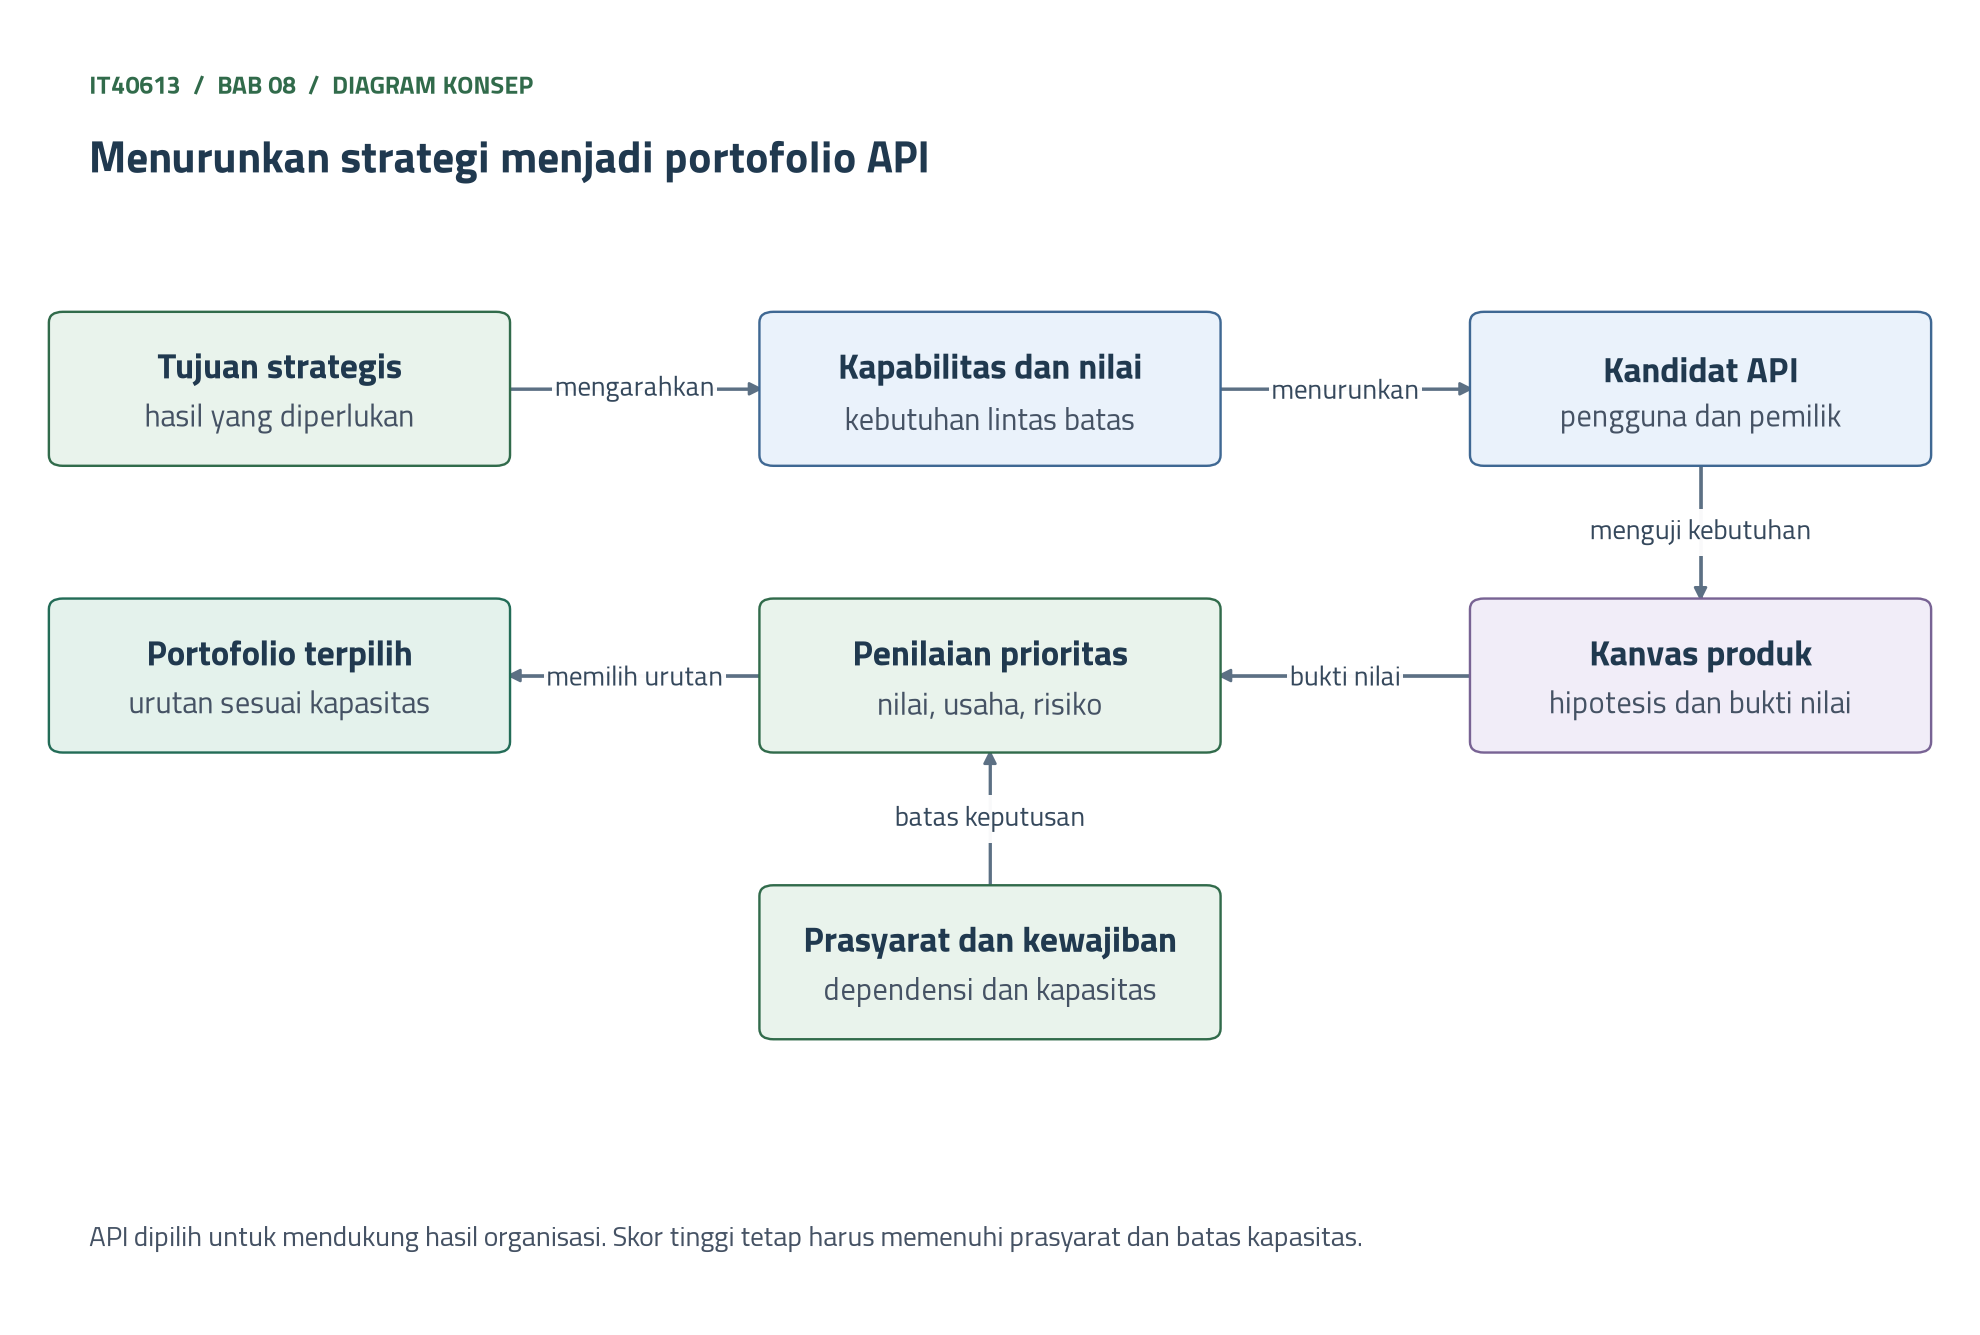
\includegraphics[width=0.96\textwidth,height=0.77\textheight,keepaspectratio]{../../figures/ch08-diagram-konsep.png}
\end{frame}

\begin{frame}{{\Large Membuka C3: Masukan dari Tonggak C2}}
  \footnotesize
  \begin{tabularx}{\textwidth}{>{\raggedright\arraybackslash}p{1.5cm}
      >{\raggedright\arraybackslash}p{3.3cm} >{\raggedright\arraybackslash}X >{\raggedright\arraybackslash}p{2.7cm}}
    \hline
    \textbf{Asal} & \textbf{Artefak} & \textbf{Temuan yang dipakai} & \textbf{Kegunaan} \\ \hline
    Bab 4 & Inventaris INT-01 sampai INT-10 & 100 sambungan, 4 baris calon produk, INT-10 tanpa pemilik & Daftar awal, biaya \\ \hline
    Bab 5 & Peta integrasi & INT-03 keterikatan, INT-02 gagal senyap, INT-06 kerja ulang & Bukti masalah \\ \hline
    Bab 6 & Penilaian keamanan & 138 tabel berlebih, layanan identitas Rp45 juta per tahun & Prasyarat, risiko \\ \hline
    Bab 7 & Kesiapan interoperabilitas & Skor 5 dari 14, KI-02 didahulukan & Kewajiban \\ \hline
    IT40513 & \textit{Capability map}, \textit{value stream} & Kode CAP, enam tahap, 2.150 keluhan & Sumber kandidat \\ \hline
  \end{tabularx}

  \vspace{8pt}
  \small 20 sambungan aktif: Rp900 juta per tahun pada Rp45 juta per antarmuka. Kerja manual: 357 jam per bulan, Rp257,04 juta per tahun.
\end{frame}

\section{Strategi API}

\begin{frame}{{\Large Strategi API Bukan Daftar API}}
  \vspace{8pt}
  \begin{itemize}
    \item Strategi API menerjemahkan tujuan platform menjadi kemampuan yang dapat dikonsumsi pihak tertentu.
    \item Tujuan menyebut hasil organisasi, pengguna, dan perubahan perilakunya.
    \item Jumlah API bukan strategi. Kandidat harus dapat ditelusuri ke masalah dan ukuran hasil.
    \item Keputusan tidak membuka suatu kemampuan juga bagian dari strategi.
  \end{itemize}
  \vspace{6pt}
  {\small Analogi: daftar menu mengikuti kebutuhan pelanggan dan kemampuan dapur, bukan seluruh bahan yang tersedia.}
\end{frame}

\begin{frame}{{\Large Dua Contoh Berangka}}
  \vspace{8pt}
  \begin{itemize}
    \item Tujuan pemesanan klinik: pencarian layanan, verifikasi syarat, dan pemesanan dinilai sebagai satu perjalanan.
    \item 40 klinik $\times$ 180 panggilan = 7.200 per hari, atau 60 persen dari kapasitas 12.000 pada kuota 300 per hari per klinik.
    \item Ukurannya janji terkonfirmasi, bukan jumlah \textit{endpoint}.
    \item Misalkan vendor analitik meminta API unduh seluruh data pasien: sekitar 1,2 juta kunjungan per tahun. Ditolak bila tanpa tujuan sah.
    \item Insiden 2025: 1.240 rekam, biaya langsung Rp23,7 juta.
  \end{itemize}
\end{frame}

\begin{frame}{{\Large Membaca Bukti Empiris dengan Hati-hati}}
  \footnotesize
  \begin{tabularx}{\textwidth}{>{\raggedright\arraybackslash}p{2.8cm} >{\raggedright\arraybackslash}X >{\raggedright\arraybackslash}p{4.1cm}}
    \hline
    \textbf{Sumber} & \textbf{Temuan} & \textbf{Batas} \\ \hline
    Benzell dkk.\ 2024 & API publik: tambahan 38,7 persen selama 16 tahun. API internal tidak signifikan. Risiko kebocoran naik & Perusahaan tercatat di bursa \\ \hline
    Wulf dan Blohm 2020 & 152 manajer produk API: strategi nilai memoderasi hubungan rancangan API dan hasil & Hanya API publik \\ \hline
    Postman 2025 & 65 persen memperoleh pendapatan, 34 persen tidak menemukan API yang sudah ada & Penerbit menjual alat API \\ \hline
  \end{tabularx}

  \vspace{8pt}
  \small Pelajaran: selaraskan API dengan tujuan bisnis. Jumlah API tanpa keterlihatan dapat menjadi beban.
\end{frame}

\begin{frame}{{\Large Sasaran Strategi Menjadi Kemampuan}}
  \footnotesize
  \begin{tabularx}{\textwidth}{>{\raggedright\arraybackslash}p{2.7cm}
      >{\raggedright\arraybackslash}X >{\raggedright\arraybackslash}p{2.8cm} >{\raggedright\arraybackslash}p{2.9cm}}
    \hline
    \textbf{Sasaran} & \textbf{Hasil yang diukur} & \textbf{Kemampuan} & \textbf{Batas} \\ \hline
    Layanan terintegrasi & Misalkan janji temu naik dari 28.000 menjadi 35.000 per bulan & Jadwal, pemesanan & Tanpa isi rekam medis \\ \hline
    Ekosistem mitra & 40 klinik mitra aktif, Rp1,44 miliar per tahun & Pemesanan, hasil pemeriksaan & Hanya pasien klinik itu \\ \hline
    Kepatuhan & Akses vendor dari 140 menjadi 2 tabel & Identitas, akses, status kiriman & Tanpa ekspor massal \\ \hline
    Modernisasi & Tujuan baru Rp45 juta, bukan Rp225 juta per tahun & Lapisan sistem & Tanpa nama tabel \\ \hline
  \end{tabularx}

  \vspace{8pt}
  \small Strategi platform: siapa bertemu siapa. Strategi API: kemampuan mana, untuk siapa, batas apa, urutan apa.
\end{frame}

\section{Menurunkan Kandidat}

\begin{frame}{{\Large Dari Kapabilitas, Bukan dari Daftar Sistem}}
  \vspace{8pt}
  \begin{itemize}
    \item \textit{Capability map}: kemampuan bisnis. \textit{Value stream}: rangkaian nilai dari sudut pengguna.
    \item Kapabilitas memungkinkan tahap dalam \textit{value stream} berjalan.
    \item Kandidat muncul ketika kemampuan perlu dipakai lintas batas.
    \item Daftar sistem hanya menunjukkan lokasi implementasi sekarang.
    \item Tiga uji: lintas batas, pengguna nyata, bukti masalah.
  \end{itemize}
  \vspace{6pt}
  {\small Analogi: nama loket mengikuti layanan, bukan merek komputer petugas.}
\end{frame}

\begin{frame}{{\Large Penurunan Kandidat pada Value Stream}}
  \centering
  \eadiagram{../../figures/ch08-penurunan-kandidat.tex}
\end{frame}

\begin{frame}{{\Large Dua Contoh Berangka}}
  \vspace{8pt}
  \begin{itemize}
    \item Dari daftar sistem: 5 API jadwal, 200 sambungan di sisi klinik, Rp225 juta per tahun.
    \item Dari kapabilitas CAP-L03: 1 API dan 5 adaptor, 40 sambungan, Rp270 juta per tahun.
    \item Misalkan 5 perubahan per tahun: 800 jam, Rp48 juta di sisi klinik. Selisih Rp45 juta tertutup.
    \item INT-03: vendor membaca 140 tabel, kebutuhan 2 tabel. Akses atas 138 tabel dihapus.
    \item Keluhan tahap 2 dan 3: 1.360 dari 2.150, sekitar 63 persen. Keluhan belum menunjukkan penyebab.
  \end{itemize}
\end{frame}

\begin{frame}{{\Large Delapan Kandidat API Medikara}}
  \scriptsize
  \begin{tabularx}{\textwidth}{>{\raggedright\arraybackslash}p{1.15cm} >{\raggedright\arraybackslash}p{3.1cm}
      >{\raggedright\arraybackslash}p{1.55cm} >{\raggedright\arraybackslash}X >{\raggedright\arraybackslash}p{3.3cm}}
    \hline
    \textbf{ID} & \textbf{Kandidat} & \textbf{Kapabilitas} & \textbf{Baris dan bukti} & \textbf{Pemilik} \\ \hline
    API-01 & Jadwal dan Janji Temu & CAP-L03 & INT-03: 28.000 janji temu per bulan & Manajer Layanan Rawat Jalan \\ \hline
    API-02 & Hasil Pemeriksaan & CAP-L06 & INT-06, Bab 5: 110 jam, 72 telepon per hari & Manajer Laboratorium \\ \hline
    API-03 & Klaim Asuransi & CAP-P01 & INT-05: 468 klaim ditolak per bulan & Manajer Klaim \\ \hline
    API-04 & Rekap Perusahaan & Belum ada & INT-07: 36 rekap, 32 jam per bulan & Manajer Layanan Perusahaan \\ \hline
    API-05 & Rekap Klinik & CAP-P03 & INT-09: 48 jam per bulan & Manajer Pelaporan \\ \hline
    API-06 & Identitas dan Akses & CAP-P02 & Bab 6: diperlukan tiga integrasi & Kepala Keamanan Informasi \\ \hline
    API-07 & Mutasi Bank & CAP-P04 & INT-08: 50 jam per bulan & Manajer Keuangan \\ \hline
    API-08 & Resep Apotek & CAP-L06 & INT-10: volume belum diketahui & Belum ada \\ \hline
  \end{tabularx}
\end{frame}

\begin{frame}{{\Large Kasus Medikara: Menerjemahkan Permintaan}}
  \vspace{8pt}
  \begin{itemize}
    \item Vendor meminta tabel tambahan. Kebutuhannya kemampuan penjadwalan.
    \item Dua asuransi meminta format masing-masing. Digabung menjadi satu kandidat, API-03.
    \item API-08 lolos uji lintas batas, gagal uji bukti. Tetap ditulis supaya tidak hilang.
    \item Verifikasi penjaminan Rp960 juta: kandidat lanjutan, karena kontrak 9 asuransi belum ada.
    \item Identitas pemanggil (API-06) berbeda dari identitas pasien (MPI, hipotesis KI-03).
  \end{itemize}
\end{frame}

\section{Domain dan Lapisan}

\begin{frame}{{\Large Batas Domain dan Tiga Lapisan}}
  \vspace{8pt}
  \begin{itemize}
    \item Batas domain mengelompokkan makna dan aturan bisnis yang konsisten.
    \item \textit{Bounded context}: batas tempat sebuah model didefinisikan dan berlaku.
    \item Lapisan sistem, proses, dan pengalaman membedakan tanggung jawab, bukan kewajiban tiga lapisan fisik.
    \item Istilahnya berasal dari sisi vendor: \textit{API-led connectivity}. Dipakai sebagai alat berpikir.
    \item Analisis domain rinci dibahas di IT40713.
  \end{itemize}
  \vspace{6pt}
  {\small Analogi: formulir lintas bagian tanpa penanggung jawab terus membengkak.}
\end{frame}

\begin{frame}{{\Large Lapisan pada Tiga Kandidat}}
  \centering
  \eadiagram{../../figures/ch08-lapisan-api.tex}
\end{frame}

\begin{frame}{{\Large Alasan Berubah Menentukan Lapisan}}
  \footnotesize
  \begin{tabularx}{\textwidth}{>{\raggedright\arraybackslash}p{2.0cm}
      >{\raggedright\arraybackslash}X >{\raggedright\arraybackslash}p{2.7cm} >{\raggedright\arraybackslash}p{2.9cm}}
    \hline
    \textbf{Lapisan} & \textbf{Tanggung jawab} & \textbf{Berubah karena} & \textbf{Contoh} \\ \hline
    Pengalaman & Menyajikan data untuk satu kanal & Kebutuhan kanal & Tampilan Medikara+ \\ \hline
    Proses & Menjalankan aturan lintas langkah & Aturan bisnis & Pemesanan \\ \hline
    Sistem & Menyembunyikan sistem sumber & Vendor atau versi & Adaptasi SIMRS \\ \hline
  \end{tabularx}

  \vspace{8pt}
  \begin{itemize}
    \small
    \item Aturan kunci slot disalin ke Medikara+ dan 40 klinik: 41 salinan, 41 pekerjaan per perubahan.
    \item Tujuan baru: langsung Rp225 juta, lewat lapisan Rp45 juta per tahun.
    \item Lapisan bersama Rp300 juta: empat tujuan Rp705 juta dibanding Rp900 juta.
  \end{itemize}
\end{frame}

\section{Lanskap API}

\begin{frame}{{\Large Delapan Aspek Lanskap API}}
  \scriptsize
  \begin{tabularx}{\textwidth}{>{\raggedright\arraybackslash}p{1.9cm} >{\raggedright\arraybackslash}X >{\raggedright\arraybackslash}p{4.7cm}}
    \hline
    \textbf{Aspek} & \textbf{Keadaan Medikara} & \textbf{Akibat pada portofolio} \\ \hline
    \textit{Variety} & Enam cara bertukar data pada sepuluh baris & Gaya baru dibatasi \\ \hline
    \textit{Vocabulary} & Kunjungan, janji temu, Encounter tertukar & Kosakata sebelum kontrak Bab 9 \\ \hline
    \textit{Volume} & 100 sambungan, 10 lewat API, 0 API mitra & Peninjauan terpusat masih memadai \\ \hline
    \textit{Velocity} & 4 pembaruan pihak wajib, 18 perubahan asuransi & API-03 beban perubahan tertinggi \\ \hline
    \textit{Vulnerability} & Jadwal kosong 7 sampai 14 hari per tahun & API-01 wajib punya rencana cadangan \\ \hline
    \textit{Visibility} & INT-10 tanpa pemilik, INT-02 gagal senyap & Telemetri syarat tiap API baru \\ \hline
    \textit{Versioning} & Tiap pembaruan diterapkan lima kali & Kebijakan versi di Bab 10 \\ \hline
    \textit{Volatility} & 138 tabel berlebih, insiden 1.240 rekam & API-06 menjadi prasyarat \\ \hline
  \end{tabularx}

  \vspace{6pt}
  {\footnotesize Pemaknaan \textit{vulnerability} dan \textit{volatility} mengikuti ringkasan Amundsen. Gangguan dan keamanan diperiksa bersama.}
\end{frame}

\begin{frame}{{\Large Lanskap Berbeda dari Portofolio}}
  \vspace{8pt}
  \begin{itemize}
    \item Lanskap: seluruh API dan integrasi yang ada, termasuk milik pihak lain.
    \item Portofolio: pilihan investasi atas kandidat yang dapat diputuskan organisasi.
    \item Misalkan SIMRS, Medikara+, dan SATUSEHAT memaknai kunjungan berbeda: 100.000, 55.000, dan 28.000 per bulan tampak seperti satu ukuran.
    \item INT-10: 12 sambungan tanpa pemilik. Misalkan penelusuran 2 jam per apotek: 24 jam, Rp1,44 juta.
  \end{itemize}
  \vspace{6pt}
  {\small Analogi: pengelola kota memerlukan peta kepadatan dan rencana perubahan, bukan hanya daftar nama jalan.}
\end{frame}

\section{Kanvas dan Pemilik}

\begin{frame}{{\Large Kanvas Produk API}}
  \vspace{8pt}
  \begin{itemize}
    \item Delapan unsur: pengguna, masalah, tawaran nilai, operasi, dependensi, risiko, ukuran, pemilik.
    \item Kanvas adalah hipotesis, diuji lewat percakapan dan percobaan.
    \item Bentuk satu halaman berasal dari \textit{Business Model Canvas}.
    \item Versi singkat sebelum skor: pengguna, masalah, ukuran, pemilik.
    \item Versi lengkap sesudah skor, untuk dua atau tiga kandidat teratas.
  \end{itemize}
  \vspace{6pt}
  {\small Analogi: proposal satu halaman memeriksa apakah masalah dan tawarannya sesuai.}
\end{frame}

\begin{frame}{{\Large Kanvas API-01}}
  \centering
  \eadiagram{../../figures/ch08-kanvas-produk.tex}
\end{frame}

\begin{frame}{{\Large Dua Contoh Berangka}}
  \vspace{8pt}
  \begin{itemize}
    \item 40 klinik $\times$ 60 kunjungan = 2.400 pemesanan per hari. Misalkan 10 persen diikuti telepon 3 menit.
    \item Beban 300 jam per bulan, Rp216 juta per tahun. Bila telepon tidak turun, hipotesis salah.
    \item INT-06: 13.200 hasil per tahun. Misalkan 0,5 persen salah ketik: 66 hasil keliru.
    \item API memindahkan risiko ke pencocokan pasien: 72.000 hasil, 1 dari 10.000, sekitar 7 salah sasaran.
    \item Karena itu notifikasi Bab 5 tidak memuat isi hasil.
  \end{itemize}
\end{frame}

\begin{frame}{{\Large Pemilik Produk API}}
  \footnotesize
  \begin{tabularx}{\textwidth}{>{\raggedright\arraybackslash}p{2.75cm}
      >{\raggedright\arraybackslash}X >{\raggedright\arraybackslash}X >{\raggedright\arraybackslash}p{2.35cm} >{\raggedright\arraybackslash}p{2.35cm}}
    \hline
    \textbf{Keputusan} & \textbf{Pemilik produk} & \textbf{Tim integrasi} & \textbf{Vendor} & \textbf{Keamanan} \\ \hline
    Prioritas perubahan & Memutuskan & Memberi perkiraan & Memberi masukan & Dimintai pendapat \\ \hline
    Anggaran, ukuran & Memutuskan & Melaporkan data & Tidak terlibat & Tidak terlibat \\ \hline
    Kontrak, operasi & Menyetujui yang besar & Memutuskan & Mengikuti kontrak & Meninjau \\ \hline
    Hak akses, \textit{scope} & Menyetujui kebutuhan & Menerapkan & Mengikuti & Memutuskan \\ \hline
  \end{tabularx}

  \vspace{6pt}
  \small API-01: Manajer Layanan Rawat Jalan. Vendor bukan otomatis pemilik: 18 perubahan $\times$ Rp8 juta = Rp144 juta per tahun. Misalkan 12 perubahan per triwulan, kapasitas 6: pemilik memilih.
\end{frame}

\section{Prioritisasi Portofolio}

\begin{frame}{{\Large Skor Tidak Menggantikan Kewajiban}}
  \vspace{8pt}
  \begin{itemize}
    \item Prioritisasi menggabungkan nilai, usaha, risiko, dependensi, dan kapasitas.
    \item Bobot dan skala disepakati sebelum skor diisi.
    \item Cooper dkk.: 205 perusahaan. Kelompok terbaik memakai prosedur formal, lebih dari satu metode, dan menekankan metode strategis.
    \item Metode keuangan yang paling populer memberi hasil lebih buruk. Studinya tentang produk baru, bukan API.
  \end{itemize}
  \vspace{6pt}
  {\small Analogi: dapur yang paling diinginkan tetap menunggu pipa air.}
\end{frame}

\begin{frame}{{\Large Peta Keputusan Portofolio}}
  \centering
  \eadiagram{../../figures/ch08-peta-keputusan.tex}
\end{frame}

\begin{frame}{{\Large Skala Penilaian}}
  \footnotesize
  \begin{tabularx}{\textwidth}{>{\raggedright\arraybackslash}p{0.9cm} >{\raggedright\arraybackslash}p{4.3cm}
      >{\raggedright\arraybackslash}p{2.9cm} >{\raggedright\arraybackslash}X}
    \hline
    \textbf{Skor} & \textbf{Nilai per tahun} & \textbf{Usaha} & \textbf{Risiko} \\ \hline
    5 & Minimal Rp500 juta & Lebih dari 3.000 jam & Hasil klinis per pasien ke luar \\ \hline
    4 & Rp150 juta sampai kurang dari Rp500 juta & 2.001 sampai 3.000 jam & Data klinis ke mitra terkontrak \\ \hline
    3 & Rp50 juta sampai kurang dari Rp150 juta & 1.001 sampai 2.000 jam & Data pribadi terbatas, kredensial \\ \hline
    2 & Di bawah Rp50 juta & 501 sampai 1.000 jam & Data operasional \\ \hline
    1 & Tanpa manfaat langsung terukur & Sampai 500 jam & Data publik \\ \hline
  \end{tabularx}

  \vspace{8pt}
  \small Rupiah dan jam menjadi batas skala, supaya dua penilai tidak menafsirkan angka 4 secara berbeda.
\end{frame}

\begin{frame}{{\Large Skor Lima Kandidat}}
  \footnotesize
  \begin{tabularx}{\textwidth}{>{\raggedright\arraybackslash}p{3.7cm} >{\raggedright\arraybackslash}p{0.9cm}
      >{\raggedright\arraybackslash}p{0.95cm} >{\raggedright\arraybackslash}p{0.95cm} >{\raggedright\arraybackslash}p{0.8cm}
      >{\raggedright\arraybackslash}X >{\raggedright\arraybackslash}p{1.0cm}}
    \hline
    \textbf{Kandidat} & \textbf{Nilai} & \textbf{Usaha} & \textbf{Risiko} & \textbf{Skor} & \textbf{Dasar nilai per tahun} & \textbf{Jam} \\ \hline
    API-01 Janji Temu & 5 & 4 & 3 & 3,7 & Rp1,44 miliar langganan & 2.400 \\ \hline
    API-02 Hasil & 4 & 4 & 5 & 2,8 & Hingga Rp208,8 juta & 2.400 \\ \hline
    API-04 Rekap Perusahaan & 2 & 2 & 3 & 2,8 & Rp23,04 juta & 800 \\ \hline
    API-03 Klaim & 3 & 5 & 4 & 2,2 & Rp56,16 juta & 4.167 \\ \hline
    API-06 Identitas & 1 & 3 & 3 & 2,0 & Tanpa manfaat langsung & 1.200 \\ \hline
  \end{tabularx}

  \vspace{8pt}
  \small Bobot: nilai 50, usaha 30, risiko 20 persen. Usaha dan risiko dibalik: 6 dikurangi skor. Misalnya API-01: 0,5 $\times$ 5 + 0,3 $\times$ 2 + 0,2 $\times$ 3 = 3,7.
\end{frame}

\begin{frame}{{\Large Matriks Nilai dan Usaha}}
  \centering
  \eadiagram{../../figures/ch08-matriks-nilai-usaha.tex}
\end{frame}

\begin{frame}{{\Large Kapasitas Menentukan Batas}}
  \footnotesize
  \begin{tabularx}{\textwidth}{>{\raggedright\arraybackslash}p{1.2cm} >{\raggedright\arraybackslash}X
      >{\raggedright\arraybackslash}p{1.3cm} >{\raggedright\arraybackslash}p{2.0cm} >{\raggedright\arraybackslash}p{1.6cm}}
    \hline
    \textbf{Urutan} & \textbf{Pekerjaan} & \textbf{Jam} & \textbf{Biaya} & \textbf{Sisa jam} \\ \hline
    1 & Kewajiban INT-02: KI-01 dan KI-02 & 600 & Rp36 juta & 7.080 \\ \hline
    2 & API-06 Identitas dan Akses & 1.200 & Rp72 juta & 5.880 \\ \hline
    3 & API-01 Jadwal dan Janji Temu & 2.400 & Rp144 juta & 3.480 \\ \hline
    4 & API-02 Hasil Pemeriksaan & 2.400 & Rp144 juta & 1.080 \\ \hline
    & \textbf{Jumlah, sekitar 86 persen} & \textbf{6.600} & \textbf{Rp396 juta} & \textbf{1.080} \\ \hline
  \end{tabularx}

  \vspace{8pt}
  \small Misalkan 4 orang $\times$ 160 jam $\times$ 12 bulan = 7.680 jam, atau Rp460,8 juta pada tarif Rp60.000 per jam. API-04 masih muat, tetapi cadangan turun dari 14 ke sekitar 4 persen. API-03 kurang 3.087 jam. Cadangan belum final: Bab 10, 11, dan 13 memakainya, lalu Bab 14 menggeser 2.000 jam API-02 ke 2028.
\end{frame}

\begin{frame}{{\Large Membangun, Membeli, atau Memakai}}
  \footnotesize
  \begin{tabularx}{\textwidth}{>{\raggedright\arraybackslash}p{2.5cm}
      >{\raggedright\arraybackslash}X >{\raggedright\arraybackslash}p{3.1cm} >{\raggedright\arraybackslash}p{2.8cm}}
    \hline
    \textbf{Pilihan} & \textbf{Cocok bila} & \textbf{Biaya dihitung} & \textbf{Contoh} \\ \hline
    Membangun sendiri & Khusus bagi satu hubungan & Jam dan perawatan & API-01, API-02 \\ \hline
    Membeli & Kemampuan umum, pasarnya tersedia & Langganan, biaya keluar & API-06 \\ \hline
    Memakai API pihak lain & Pihak lain memiliki data atau aturan & Adaptasi, perubahan sepihak & INT-01, INT-02, API bank \\ \hline
  \end{tabularx}

  \vspace{8pt}
  \begin{itemize}
    \small
    \item INT-08: kerja manual Rp36 juta, satu antarmuka Rp45 juta per tahun. API bank belum menang.
    \item API-06, tiga tahun: membangun Rp207 juta. Misalkan membeli Rp204 juta. Penentunya kendali dan 800 jam terbebas.
  \end{itemize}
\end{frame}

\begin{frame}{{\Large Kasus Medikara: Portofolio API Target}}
  \scriptsize
  \begin{tabularx}{\textwidth}{>{\raggedright\arraybackslash}p{1.7cm} >{\raggedright\arraybackslash}p{4.0cm}
      >{\raggedright\arraybackslash}X}
    \hline
    \textbf{Status} & \textbf{Butir} & \textbf{Alasan} \\ \hline
    Kewajiban & INT-02: KI-01 dan KI-02 & Tanpa skor. Tumpukan Rp240 juta per tahun bila dibiarkan \\ \hline
    Tahun depan & API-06 Identitas dan Akses & Prasyarat API-01 dan API-02 \\ \hline
    Tahun depan & API-01 Jadwal dan Janji Temu & Skor 3,7, interaksi inti, temuan audit \\ \hline
    Tahun depan & API-02 Hasil Pemeriksaan & Skor 2,8, manfaat hingga Rp208,8 juta \\ \hline
    Antrean & API-03, API-04 & Rp250 juta untuk Rp56,16 juta, dengan perawatan teknis Rp45 juta atau produk penuh Rp180 juta (Bab 4); Rp23,04 juta di bawah Rp45 juta \\ \hline
    Dirapikan & API-05, API-07 & Manfaat di bawah Rp45 juta per tahun \\ \hline
    Ditelusuri & API-08 Resep Apotek & Tanpa pemilik, tanpa volume \\ \hline
    Ditolak & Unduh seluruh data pasien & Tanpa tujuan sah \\ \hline
  \end{tabularx}
\end{frame}

\begin{frame}{{\Large Biaya dan Konsekuensi Portofolio}}
  \vspace{8pt}
  \begin{itemize}
    \item Tahun pertama: pembangunan Rp396 juta dan perawatan 3 antarmuka Rp135 juta, jumlah Rp531 juta.
    \item Lapisan bersama Rp300 juta per tahun dicatat terpisah, dirancang di Bab 10. Bila dipasang: Rp831 juta.
    \item Bab 9 menulis kontrak untuk API-01.
    \item 468 klaim per bulan tetap ditolak: 117 jam per bulan, Rp84,24 juta per tahun. Masalah ini sengaja ditanggung.
    \item Bobot risiko naik: API-02 turun dari posisi kedua bersama API-04 ke posisi ketiga.
  \end{itemize}
\end{frame}

\section{Aktivitas}

\begin{frame}{{\Large Aktivitas: Tujuan dan Peran}}
  \vspace{6pt}
  \begin{itemize}
    \item Tujuan: menurunkan dan memprioritaskan kandidat API menjadi artefak C3 yang dapat ditelusuri.
    \item Latar bisnis, kesehatan, hukum, atau akuntansi: menilai nilai bagi pengguna dan mitra, serta kewajiban.
    \item Latar teknis: menilai usaha, ketergantungan sistem, dan risiko.
    \item Koordinator mencatat keputusan. Penelaah menantang asumsi tanpa mengganti bukti dengan pendapat.
  \end{itemize}
  \vspace{4pt}
  {\small Data organisasi nyata seizin organisasi dan dianonimkan. Data pribadi pasien atau karyawan tidak boleh dipakai.}
\end{frame}

\begin{frame}{{\Large Aktivitas: Langkah dan Luaran}}
  \vspace{4pt}
  \begin{enumerate}
    \item Ambil kapabilitas, perjalanan pengguna, dan temuan C2.
    \item Daftarkan lima sampai delapan kandidat, isi kanvas singkat.
    \item Lewatkan tiga gerbang, sepakati skala dan bobot.
    \item Gambar matriks, hitung sisa kapasitas.
    \item Isi kanvas lengkap untuk dua atau tiga kandidat, tulis portofolio.
  \end{enumerate}
  \vspace{4pt}
  {\small Luaran: portofolio API target, matriks, kanvas, catatan alternatif, tautan bukti. Membuka C3. Bobot: konsep 25, bukti 30, alasan 30, keterbacaan 15 persen. Berkas: \texttt{sources/chapter08/}.}
\end{frame}

\section{Ringkasan dan Latihan}

\begin{frame}{{\Large Ringkasan}}
  \vspace{6pt}
  \begin{itemize}
    \item Strategi API memilih kemampuan, pengguna, batas, dan urutan. Jumlah API bukan strategi.
    \item Kandidat diturunkan dari kapabilitas dan \textit{value stream}, bukan dari daftar sistem.
    \item Lapisan membedakan tanggung jawab. Lanskap memuat yang ada, portofolio memuat yang dapat diputuskan.
    \item Kanvas adalah hipotesis yang diuji. Pemilik produk menanggung akibat keputusan.
    \item API-06 berskor terendah tetap didahulukan. Masalah yang ditunda ditulis beserta akibatnya.
  \end{itemize}
\end{frame}

\begin{frame}{{\Large Latihan 1: Menurunkan Kandidat dari Kapabilitas}}
  \vspace{8pt}
  Jelaskan mengapa daftar API yang diturunkan dari daftar sistem berbeda dengan daftar API yang diturunkan dari kapabilitas bisnis.
  \vspace{6pt}
  \begin{itemize}
    \item Pilih satu kapabilitas yang dilayani lebih dari satu sistem.
    \item Tulis kedua daftar, lalu hitung sambungan dan biayanya.
    \item Jelaskan informasi vendor yang sengaja disembunyikan.
  \end{itemize}
  \vspace{4pt}
  {\small Pembanding: 200 sambungan, Rp225 juta, dan 40 sambungan, Rp270 juta.}
\end{frame}

\begin{frame}{{\Large Latihan 2: Memilih Tiga API}}
  \vspace{8pt}
  Misalkan Medikara hanya punya anggaran untuk tiga API tahun depan. Susun kriteria prioritisasi, lalu terapkan pada lima kandidat API.
  \vspace{6pt}
  \begin{itemize}
    \item Sepakati skala dan dua perangkat bobot sebelum menilai.
    \item Hitung skor pada kedua perangkat bobot.
    \item Periksa prasyarat, lalu pilih tiga API dalam batas kapasitas.
  \end{itemize}
  \vspace{4pt}
  {\small Pembanding bobot 40, 20, 40 persen: API-01 3,6; API-04 2,8; API-02 2,4; API-03 2,2; API-06 2,2.}
\end{frame}

\begin{frame}{{\Large Latihan 3: Menentukan Pemilik Produk}}
  \vspace{8pt}
  Tentukan siapa pemilik produk yang tepat untuk API janji temu Medikara, lalu jelaskan tanggung jawabnya.
  \vspace{6pt}
  \begin{itemize}
    \item Telusuri proses janji temu.
    \item Pilih pihak yang dapat memutus prioritas dan merasakan akibatnya.
    \item Pisahkan peran bisnis dan pemeliharaan teknis.
    \item Tulis jalur penyelesaian bila kebutuhan antarfasilitas berbenturan.
  \end{itemize}
\end{frame}

\end{document}
